% You should title the file with a .tex extension (hw1.tex, for example)
\documentclass[12pt]{article}\sloppy

\usepackage{amsmath,bm}
\usepackage{amssymb}
\usepackage{fancyhdr}
\usepackage{graphicx}
\usepackage{float}
\usepackage{longtable}
\usepackage{hyperref}

\floatplacement{figure}{H}
\oddsidemargin0cm
\topmargin-2cm     %I recommend adding these three lines to increase the 
\textwidth16.5cm   %amount of usable space on the page (and save trees)
\textheight23.5cm  

\newcommand{\myname}{Abhinav Maurya}
\newcommand{\myandrew}{amaurya@andrew.cmu.edu}
\newcommand{\myhwnum}{4}

\newcommand{\question}[2] {\vspace{.25in} \hrule\vspace{0.5em} \noindent{\bf #1: #2} \vspace{0.5em} \hrule \vspace{.10in}}
\renewcommand{\part}[1] {\vspace{.10in} {\bf (#1)}}

\setlength{\parindent}{0pt}
\setlength{\parskip}{5pt plus 1pt}
 
\pagestyle{fancyplain}
\lhead{\fancyplain{}{\textbf{HW\myhwnum}}}      % Note the different brackets!
\rhead{\fancyplain{}{\myname\\ \myandrew}}
\chead{\fancyplain{}{16-720}}

\begin{document}

\medskip                        % Skip a "medium" amount of space
                                % (latex determines what medium is)
                                % Also try: \bigskip, \littleskip

\thispagestyle{plain}
\begin{center}                  % Center the following lines
{\Large 16-720: Assignment \myhwnum} \\
\myname \\
\myandrew \\
\end{center}

\question{1.1}{}

Since both images are normalized, $x1 = [0,0,1]$ and $x2 = [0,0,1]$. By definition of fundamental matrix, $x2^T*F*x1=0$. By SVD, $F = U*\Sigma*V^T$. $$\therefore x2^T*U*\Sigma*V^T*x1=0$$ Considering $U = [u1;u2;u3]$ and $V=[v1;v2;v3]$, we can substitute $x1$, $x2$, $U$, and $V$ in the equation to get $$u3*sigma3*v3=0$$ If $sigma3 \neq 0$, then the relation does not hold. Hence, the smallest singular value of fundamental matrix has to be zero. 

\question{1.2}{}

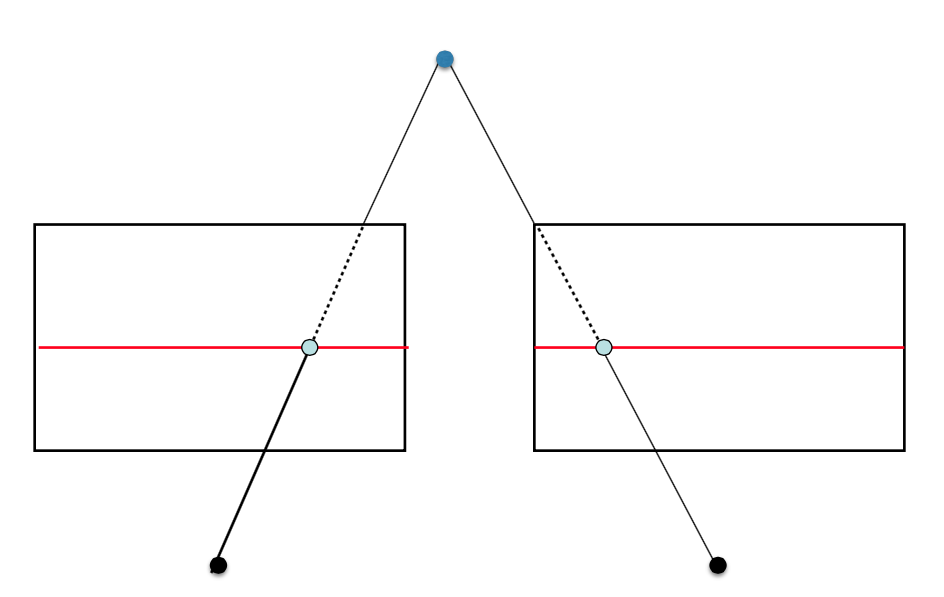
\includegraphics[width=0.8\linewidth]{fig1.png}

The case of original camera C1 and camera translated along X-axis C2 looks like figure above.

Let's consider camera intrinsic matrix to be identity since we are investigating variations in camera extrinsics (trnaslation). Let's consider the camera extrinsic matrix for C1: $[I | 0]$. $$\therefore \lambda * [x;y;1] = [I | 0] * [X;Y;Z;1]$$

For camera $C2$, the camera extrinsic matrix is $[I | t_x;0;0]$ i.e. $t_x$ translation along X-axis. $$\therefore \lambda * [x;y;1] = [I | t_x;0;0] * [X;Y;Z;1]$$ Thus, we see that the point projected on the image surfaces of cameras C1 and C2 differ only in their x-coordinate. As we vary the 3D homogeneous point $[X;Y;Z;1]$ in the epipolar plane, we trace out the epipolar line parallel to X-axis.

\question{1.3}{}

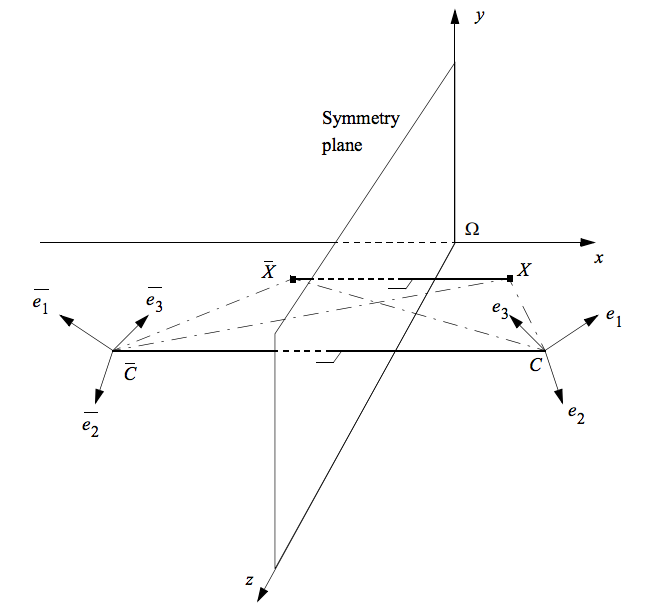
\includegraphics[width=0.8\linewidth]{fig2.png}

From the figure above which appeared in \url{http://iris.usc.edu/outlines/papers/2003/alex-ivc2003.pdf}, we see that we can place the camera along a symmetry plane from which all corresponding points of the object and its mirror image are equidistant. If this is not the case, the same rotation and translation transformation can be applied to both points and our result will still hold. Also, the camera intrinsic matrix is assumed to be identity. If it is not, its effect is identical on projections of both the object and its mirror image.

Consider point $P$ on the object and its corresponding point $Q$ in the mirror image. In the plate of the camera positioned on the symmetry plane, these points are captured at positions $p=[p_x;p_y;1]$ and $q=[q_x;q_y;1]$. We know that $\lambda * p = P$ and $\lambda * q = Q$. Moreover, since $P$ and $Q$ are on either side of the symmetry plane, they differ only in one coordinate whose axis is perpendicular to the symmetry plane, say X coordinate. $$\therefore P = [-1,0,0;0,1,0;0,0,1] * Q$$ Let $T = [-1,0,0;0,1,0;0,0,1]$ $$\therefore P=T*Q$$. $$\lambda * p = \lambda * T*Q$$. Taking cross-product with $p$, we get

$$[0,-1,p_y;1,0,-p_x;-p_y,p_x,0]*[-q_x;q_y;1] = 0$$

Taking dot-product with $[1,1,1]$ to sum over, we get 

$$[1,1,1]*[0,-1,p_y;1,0,-p_x;-p_y,p_x,0]*[-q_x;q_y;1] = 0$$

This can be reworked to

$$[p_x,p_y,1]*[0,1,-1;-1,0,1;1,-1,0]*[-q_x;q_y;1]$$

If $F=[0,1,-1;-1,0,1;1,-1,0]$, $$p=F*q'$$ where $q'=[-q_x;q_y;1]$

Thus, points $p$ and $q$ are related through a skew-symmetric fundamental matrix. The $-q_x$ in $[-q_x;q_y;1]$ indicates that the mirror image is captured by the camera as a mirror image i.e. a flipped version of the image of the original object.

\question{2.1}{eightpoint}

Included in \texttt{code/eightpoint.m} file. No refinement was used since it seemed to be causing instability in estimating $F$.

\begin{verbatim}
F =

   -0.0000   -0.0000    0.0011
   -0.0000    0.0000   -0.0000
   -0.0011    0.0000   -0.0042
\end{verbatim}

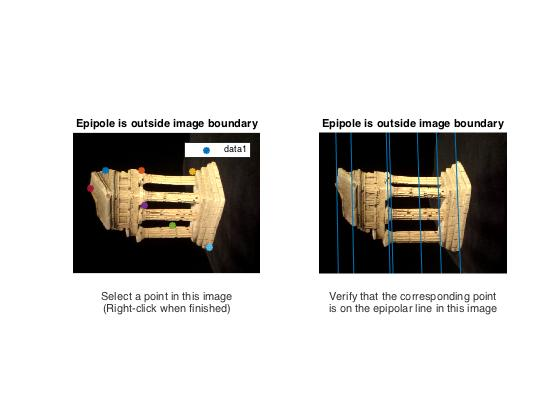
\includegraphics[width=0.8\linewidth]{fig3.jpg}

\question{2.2}{sevenpoint}

Included in \texttt{code/sevenpoint.m} file.

\begin{verbatim}
F =

    0.0000   -0.0000    0.0011
    0.0000    0.0000   -0.0001
   -0.0011    0.0001   -0.0046
\end{verbatim}

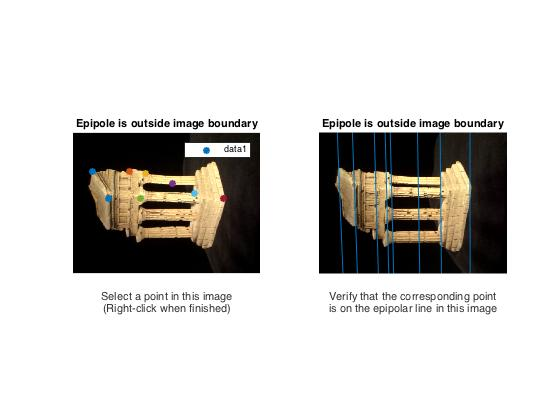
\includegraphics[width=0.8\linewidth]{fig4.jpg}

\question{2.3}{essentialMatrix}

Included in \texttt{code/essentialMatrix.m} file.

\begin{verbatim}
E =

   -0.0030   -0.3035    1.6603
   -0.1374    0.0083   -0.0512
   -1.6651   -0.0125   -0.0013
\end{verbatim}

\question{2.4}{triangulate}

Included in \texttt{code/triangulate.m} file.

\question{2.5}{findM2}

Included in \texttt{code/findM2.m} file.

\question{2.6}{epipolarCorrespondence}

Included in \texttt{code/epipolarCorrespondence.m} file. Result in figure \ref{fig:3dreconstruction}.

\question{2.7}{q2\_7}

Included in \texttt{code/q2\_7.m} file.

\begin{figure*}[f]
\centering
\begin{tabular}{c c c c}
  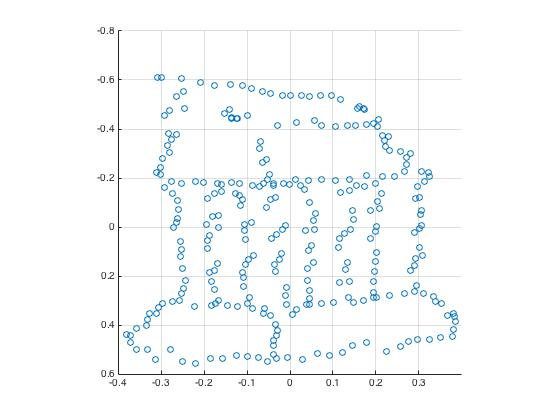
\includegraphics[trim=15mm 15mm 15mm 15mm,clip=true,width=0.23\linewidth]{fig6.jpg} & 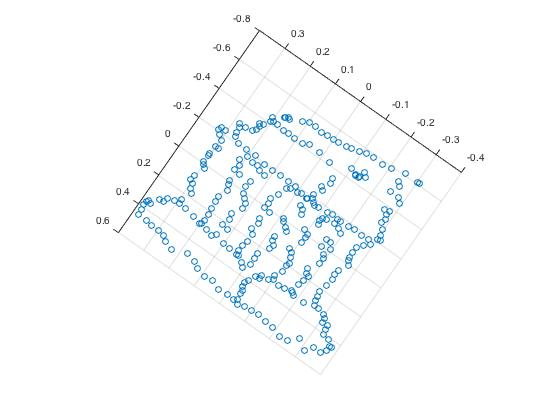
\includegraphics[trim=15mm 15mm 15mm 15mm,clip=true,width=0.23\linewidth]{fig7.jpg} & 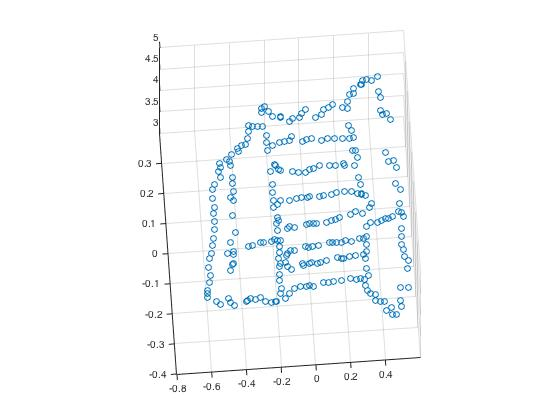
\includegraphics[trim=15mm 15mm 15mm 15mm,clip=true,width=0.23\linewidth]{fig8.jpg} & 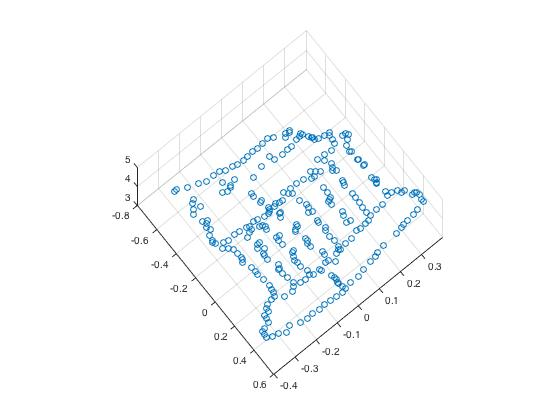
\includegraphics[trim=15mm 15mm 15mm 15mm,clip=true,width=0.23\linewidth]{fig9.jpg} \\
\end{tabular}
\caption{Output of 3D reconstruction}
\label{fig:3dreconstruction}
\end{figure*}

\end{document}

